\documentclass[bachelor, och, labwork]{shiza}

\usepackage[utf8]{inputenc}
\usepackage{graphicx}

\usepackage[sort,compress]{cite}
\usepackage{amsmath}
\usepackage{amssymb}
\usepackage{amsthm}
\usepackage{fancyvrb}
\usepackage{longtable}
\usepackage{array}
\usepackage[english,russian]{babel}
\usepackage{minted}

\usepackage{tempora}


% \usepackage[colorlinks=false]{hyperref}


\newcommand{\eqdef}{\stackrel {\rm def}{=}}


\begin{document}

\title{Алгоритмы алгебры и теории чисел}

\course{4}

\group{431}

\napravlenie{10.05.01 "--- Компьютерная безопасность}


\author{Никитина Арсения Владимировича}


\satitle{доцент}
\saname{А.\,С.\,Гераськин}


\date{2022}

\maketitle

% Включение нумерации рисунков, формул и таблиц по разделам
% (по умолчанию - нумерация сквозная)
% (допускается оба вида нумерации)
%\secNumbering


\tableofcontents

\section{Задание лабораторной работы}

Осуществить построение большого простого числа с использованием критерия Люка.

\section{Теоретическая часть}

Тест основывается на следующем критерии простоты чисел Мерсенна:

Пусть $p$ --- простое нечётное. Число Мерсенна $M_{p}=2^{p}-1$ простое тогда и 
только тогда, когда оно делит нацело $(p-1)$-й член последовательности:
$ 4,~14,~194,~37634,\;\ldots$, которая задается рекуррентно:

$$S_{k}={\begin{cases}4&k=1,\\S_{k-1}^{2}-2&k>1.\end{cases}}$$

\begin{center}
    \textit{Доказательство}
\end{center}

Один из подходов к доказательству основан на использовании функций Люка:

$${V_{n}(P,Q)=\alpha ^{n}+\beta ^{n},}$$

$$U_{n}(P,Q)={\frac {\alpha ^{n}-\beta ^{n}}{\alpha -\beta }},$$
где $\alpha ,\;\beta $  --- корни квадратного уравнения:

$$x^{2}-Px+Q=0$$
с дискриминантом $D=P^{2}-4Q$, причём $P$ и $Q$ взаимно просты.

В частности, при доказательстве используются некоторые свойства этих функций, а 
именно:

$1.~ V_{n}^{2}-DU_{n}^{2}=4Q^{n}$

$2.~ V_{2n}=V_{n}^{2}-2Q^{n},\quad U_{2n}=U_{n}V_{n}$

$3.~ {\frac {V_{n}+{\sqrt {D}}U_{n}}{2}}=\left({\frac {P+{\sqrt {D}}}{2}}\right)^{n}$

$4.~ \text{Если}~ P'\equiv P{\pmod {N}}, Q'\equiv Q{\pmod {N}}, (Q,N)=1 ~\text{и}~ QP'=P^{2}-2Q{\pmod {N}},$ то:\\

 ${\begin{cases}Q^{n}V_{n}(P',1)\equiv V_{2n}(P,Q){\pmod {N}}\\PQ^{n-1}U_{n}(P',1)\equiv U_{2n}(P,Q){\pmod {N}}\end{cases}}$\\

$5.$  Если $p$ --- простое, такое, что $2DQ$ взаимно просто с $p$, то $p$ делит нацело 
$U_{\Phi (p)}(P,Q)$, где $\Phi (p)=p-\left({\frac {D}{p}}\right)$, а $\left({\frac {D}{p}}\right)$ --- 
символ Лежандра.

\begin{center}
    \textit{Необходимость}
\end{center}

Из свойства 4. по модулю $N=M_{p}$ при $P=2$, $Q=-2$, следует:

$2^{n}V_{n}(-4,1)\equiv V_{2n}(2,-2){\pmod {N}}$,
а по свойству 2.

$V_{2n}(-4,1)=V_{n}^{2}(-4,1)-2$,
поэтому

$S_{p-1}\equiv V_{\frac {N+1}{4}}(-4,1){\pmod {N}}$
и

$V_{\frac {N+1}{2}}(2,-2)\equiv 2^{\frac {N+1}{4}}S_{p-1}{\pmod {N}}$

$D=2^{2}-4\cdot (-2)=12$, поэтому если $N$ --- простое, то 
$\left({\frac {D}{N}}\right)=-1$ и из последних двух свойств $N$ делит
$U_{N+1}(2,-2)=V_{\frac {N+1}{2}}(2,-2)U_{\frac {N+1}{2}}(2,-2)$

Далее, из свойств 1. и 2.

$V_{N+1}=V_{\frac {N+1}{2}}^{2}-2\cdot (-2)^{\frac {N+1}{2}}\equiv 8+4=12{\pmod {N}}$,
но по свойству 3 имеем:

$V_{N+1}\equiv 2(1+{\sqrt {3}})^{N+1}=2(1+{\sqrt {3}})(1+3^{\frac {N-1}{2}}{\sqrt {3}})\equiv 2(1-3)=-4{\pmod {N}}$,
то есть $N$ делит $V_{\frac {N+1}{2}}(2,-2)$, а значит и $S_{p-1}$.

\begin{center}
    \textit{Достаточность}
\end{center}

Если $N$ делит $S_{p-1}$, то из доказательства необходимости следует, что оно 
делит и $V_{\frac {N+1}{2}}$. $N$ взаимно просто с $U_{\frac {N+1}{2}}$ по свойству 1., 
а по свойству 2. --- делит $U_{N+1}$. Но тогда каждый простой делитель числа $N$ 
представим в виде $\pm 1+k2^{p}>{\sqrt {N}}$, то есть $N=M_{p}$ --- простое.


\section{Практическая часть}
\subsection{Пример работы алгоритма}
\begin{figure}[H]
    \centering
    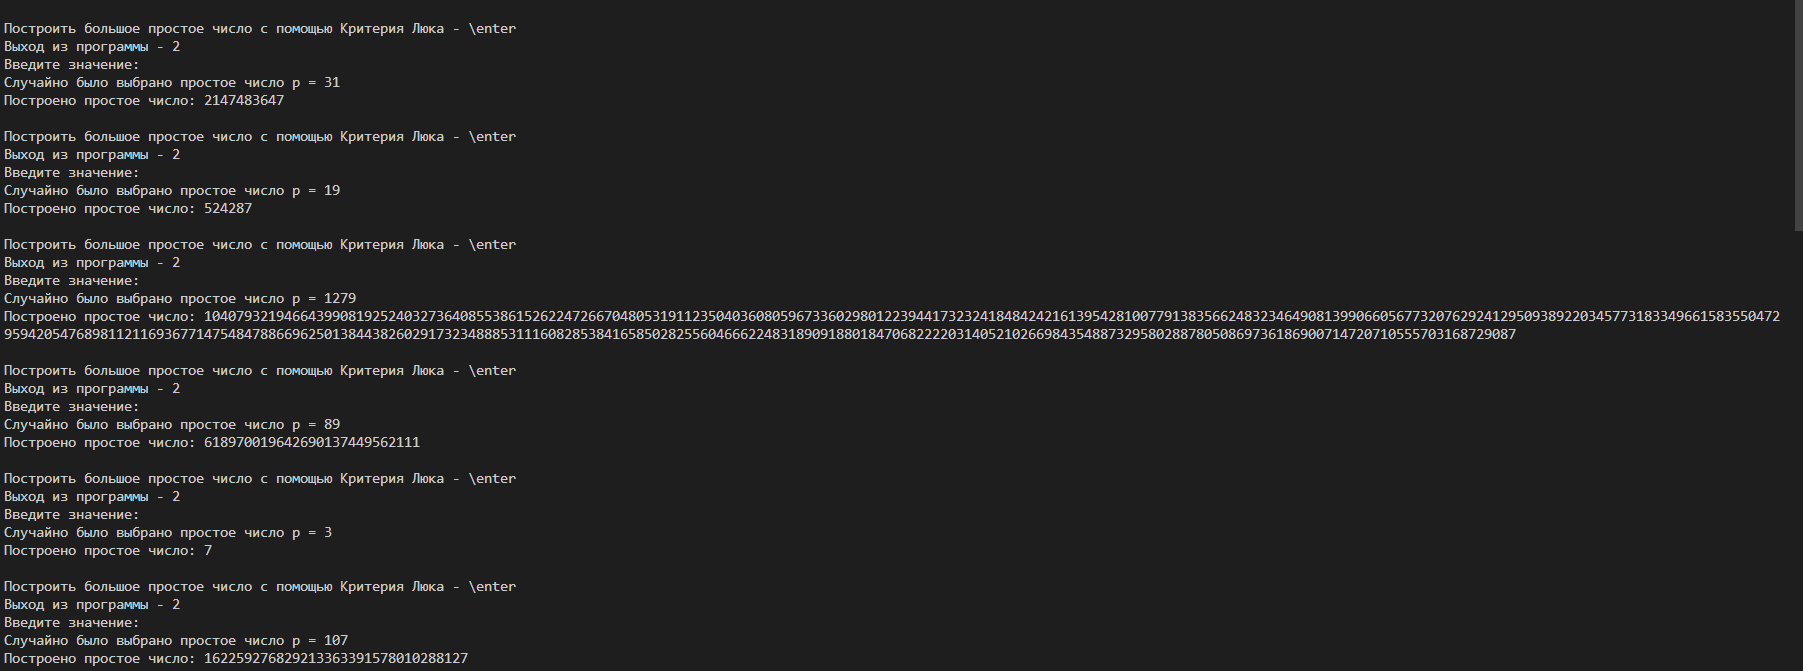
\includegraphics[width=1\textwidth]{pic1.png}
    \caption{}
\end{figure}

\setminted[python]{linenos,breaklines=true, fontsize=\small, style=bw}
    \subsection{Код программы, реализующей рассмотренный алгоритм}
        \inputminted{python}{lab9.py}

\end{document}